\documentclass[10pt,english,aspectratio=169,handout]{beamer}

\usetheme{default}

\usepackage{xstring}
\usepackage{pgfpages}
%\makeatletter
%\IfSubStr{\@classoptionslist}{handout}
%  {\pgfpagesuselayout{2 on 1}[letterpaper,border shrink=5mm]}
%  {}
%\makeatother

\usepackage{amsmath,amssymb,amsthm}
\usepackage{stmaryrd}
\usepackage{enumerate}
\usepackage{stfloats}
\usepackage{bbm}
\usepackage{pdfpages}
\usepackage{framed}
\usepackage{tabularx}


\usepackage[most]{tcolorbox}
\tcbset{highlight math style={enhanced,
  colframe=white,colback=yellow!15,arc=8pt,boxrule=1pt,
  }}
  
\usepackage{tikz,pgf,pgfplots}
\usepackage{algorithm,algorithmic}
\usepgflibrary{shapes}
\usetikzlibrary{%
  arrows,%
  arrows.meta,
  backgrounds,
  shapes.misc,% wg. rounded rectangle
  shapes.arrows,%
  shapes,%
  calc,%
  chains,%
  matrix,%
  positioning,% wg. " of "
  scopes,%
  decorations.pathmorphing,% /pgf/decoration/random steps | erste Graphik
  shadows,%
  backgrounds,%
  fit,%
  petri,%
  quotes
}

\tikzset{background rectangle/.style={
    fill=white,
  },
  use background/.style={    
    show background rectangle
  }
}

\setbeamersize{text margin left=10mm,text margin right=35mm}

\pgfplotsset{compat=1.12}

%\usetheme{Frankfurt}
%\usecolortheme{ldpc}
\useinnertheme{rounded}
\usecolortheme{whale}
\usecolortheme{orchid}

\newcommand{\ul}[1]{\underline{#1}}
\renewcommand{\Pr}{\mathbb{P}}

%% Setup slides and notes
\makeatletter
\IfSubStr{\@classoptionslist}{handout}
  {\def\slidesonly{}}{\def\slidesnotes{}}
\makeatother

%\setbeameroption{show notes on second screen=right} % Both
\ifdefined\notesonly
  \setbeameroption{show only notes} % Only notes
\fi
\ifdefined\slidesnotes
  \setbeameroption{show notes on second screen=right} % Both
\fi
\ifdefined\slidesonly
  \setbeameroption{hide notes} % Only slides
\fi
%\setbeamertemplate{note page}{\pagecolor{yellow!5}\vfill\insertnote\vfill}

\newcommand{\getpdfpages}[2]{\begingroup
  \setbeamercolor{background canvas}{bg=}
  \addtocounter{framenumber}{1}
  \includepdf[pages={#1},%
  pagecommand={%
    \expandafter\def\expandafter\insertshorttitle\expandafter{%
      \insertshorttitle\hfill\insertframenumber\,/\,\inserttotalframenumber}}%
  ]{#2}
  \endgroup}

\newcommand{\backupbegin}{
   \newcounter{finalframe}
   \setcounter{finalframe}{\value{framenumber}}
}
\newcommand{\backupend}{
   \setcounter{framenumber}{\value{finalframe}}
}

 \setbeamercolor{bibliography entry author}{fg=black}
 \setbeamercolor{bibliography entry title}{fg=black}
 \setbeamercolor{bibliography entry location}{fg=black}
 \setbeamercolor{bibliography entry note}{fg=black}
 
 \setbeamerfont{bibliography item}{size=\footnotesize}
 \setbeamerfont{bibliography entry author}{size=\footnotesize}
 \setbeamerfont{bibliography entry title}{size=\footnotesize}
 \setbeamerfont{bibliography entry location}{size=\footnotesize}
 \setbeamerfont{bibliography entry note}{size=\footnotesize}
 \setbeamertemplate{bibliography item}{\insertbiblabel}
 
\newlength\tikzwidth
\newlength\tikzheight


\newcommand{\mc}[1]{\mathcal{#1}}
\newcommand{\mbb}[1]{\mathbb{#1}}
%\newcommand{\expt}{\mbb{E}}
%\newcommand{\dd}{\mathrm{d}}
\newcommand{\Interior}[1]{\ensuremath{{#1}^{\circ}}}
\newcommand{\Closure}[1]{\ensuremath{\overline{#1}}}
\newcommand{\Complement}[1]{\ensuremath{{#1}^{c}}}

\newcommand{\Expect}{\ensuremath{\mathrm{E}}}
\newcommand{\vecnot}{\underline}
\newcommand{\RealNumbers}{\ensuremath{\mathbb{R}}}
\newcommand{\RationalNumbers}{\mathbb{Q}}
\newcommand{\ComplexNumbers}{\mathbb{C}}
\newcommand{\Real}{\mathrm{Re}}
\newcommand{\Span}{\mathrm{span}}
\newcommand{\Rank}{\mathrm{rank}}
\newcommand{\Nullity}{\mathrm{nullity}}
\newcommand{\Trace}{\mathrm{tr}}
\newcommand{\Diag}{\mathrm{diag}}
\newcommand{\dd}{\mathrm{d}}
\DeclareMathOperator*{\esssup}{ess\,sup}

% Use < , > inner product
\newcommand{\inner}[2]{{\left\langle #1 \mskip2mu , #2 \right\rangle}}
\newcommand{\tinner}[2]{{\langle #1 \mskip1mu , #2 \rangle}}

% Use < | > inner product
%\newcommand{\inner}[2]{{\left\langle #1 \mskip2mu \middle| \mskip2mu #2 \right\rangle}}
%\newcommand{\tinner}[2]{{\langle #1 \mskip1mu | \mskip1mu  #2 \rangle}}




\def\checkmark{\tikz\fill[scale=0.4](0,.35) -- (.25,0) -- (1,.7) -- (.25,.15) -- cycle;}
\def\greencheck{{\color{green}\checkmark}}
\def\scalecheck{\resizebox{\widthof{\checkmark}*\ratio{\widthof{x}}{\widthof{\normalsize x}}}{!}{\checkmark}}
\def\xmark{\tikz [x=1.4ex,y=1.4ex,line width=.2ex, red] \draw (0,0) -- (1,1) (0,1) -- (1,0);}
\def\redx{{\color{red}\xmark}}

\renewcommand{\footnotesep}{-2pt}


\begin{document}

\title{ECE 586: Vector Space Methods \\ Lecture 15 Flip Video: Inner Product Spaces}
\author{Henry D. Pfister \\ Duke University}
\date{}
%\date{August 20th, 2020}
%\maketitle

\setbeamertemplate{navigation symbols}{}

\begin{frame}[plain]
	\titlepage
	
	\note{
		\vspace{8mm}
		\begin{enumerate}
			\setlength\itemsep{3mm}
			\color{red}
			\item Welcome to the 11th video lecture for ECE 586, Vector Space Methods. \\[2mm]
			Today, we'll finish our discussion of subspaces and bases and then move on to linear transforms.
		\end{enumerate}
	}
\end{frame}

\addtocounter{framenumber}{-1}
\setbeamertemplate{navigation symbols}{\textcolor{blue}{\footnotesize \insertframenumber ~/ \inserttotalframenumber}}



\begin{frame}{3.6: Inner-Product Spaces}
\begin{definition} \label{definition:InnerProduct}
Let $F$ be the field of real numbers or the field of complex numbers, and assume $V$ is a vector space over $F$.
An \textcolor{blue}{inner product} on $V$ is a function which assigns to each ordered pair of vectors $\vecnot{v}, \vecnot{w} \in V$ a scalar $\left\langle \vecnot{v} | \vecnot{w} \right\rangle \in F$ in such a way that for all $\vecnot{u}, \vecnot{v}, \vecnot{w} \in V$ and any scalar $s \in F$
\begin{enumerate}
\item $\left\langle \vecnot{u} + \vecnot{v} | \vecnot{w} \right\rangle
= \left\langle \vecnot{u} | \vecnot{w} \right\rangle
+ \left\langle \vecnot{v} | \vecnot{w} \right\rangle$
\item $\left\langle s \vecnot{v} | \vecnot{w} \right\rangle
= s \left\langle \vecnot{v} | \vecnot{w} \right\rangle$
\item $\left\langle \vecnot{v} | \vecnot{w} \right\rangle
= \overline{ \left\langle \vecnot{w} | \vecnot{v} \right\rangle }$, where the overbar denotes complex conjugation;
\item $\left\langle \vecnot{v} | \vecnot{v} \right\rangle \geq 0$ with equality iff $\vecnot{v} = \vecnot{0}$.
\end{enumerate}
\end{definition}

\vspace{2mm}
Note that these conditions imply that:
\begin{align*}
\left\langle s \vecnot{v} + \vecnot{w} | \vecnot{u}  \right\rangle
&= s \left\langle \vecnot{v} | \vecnot{u} \right\rangle
+ \left\langle \vecnot{w} | \vecnot{u} \right\rangle \\
\left\langle \vecnot{u} | s \vecnot{v} + \vecnot{w} \right\rangle
&= \overline{s} \left\langle \vecnot{u} | \vecnot{v} \right\rangle
+ \left\langle \vecnot{u} | \vecnot{w} \right\rangle
\end{align*}
\end{frame}

\begin{frame}{3.6: Example Inner Products}

\vspace{-2mm}

\begin{example}[Standard Inner Product on $F^n$]<1->
Consider the inner product on $F^n$ defined by \vspace{-1.5mm}
\begin{equation*}
\left\langle \vecnot{v} | \vecnot{w} \right\rangle
= \left\langle (v_1, \ldots, v_n) | (w_1, \ldots, w_n) \right\rangle
\triangleq \textstyle\sum_{j=1}^n v_j \overline{w}_j. \vspace{-1.5mm}
\end{equation*}
For column vectors, it follows that $ \left\langle \vecnot{v} | \vecnot{w} \right\rangle = \vecnot{w}^H \vecnot{v} $
\end{example}

\begin{example}[Standard Inner Product on a Function Space]<2->
Let $V$ be the vector space of all continuous complex-valued functions on the unit interval $[0,1]$.
Then, the following defines an inner product \vspace{-1.5mm}
\begin{equation*}
\left\langle f | g \right\rangle
= \textstyle\int_0^1 f(t) \overline{g(t)} \, dt
\end{equation*}
\end{example}

\begin{example}[Inner Product on Space of Random Variables]<3->
Let $W$ be a set of real-valued random variables with finite 2nd moments.
Then, $V = \Span (W)$ is a vector space over $\RealNumbers$ with inner product \vspace{-1.5mm}
\[ \left\langle X | Y \right\rangle = \Expect \left[ XY \right] \]
\end{example}


\end{frame}

\begin{frame}{3.6: Properties of the Inner Product (1)}

\vspace{-1.5mm}

\begin{theorem}
Let $V$ be a finite-dimensional space with ordered basis $\mathcal{B} = \vecnot{w}_1, \ldots, \vecnot{w}_n$.
Then, any inner product on $V$ is determined by the values \vspace{-1,5mm}
\begin{equation*}
g_{ij} = \left\langle \vecnot{w}_j | \vecnot{w}_i \right\rangle.
\end{equation*}
\end{theorem}

\begin{proof}<2->
If $\vecnot{u} = \sum_{j} s_j \vecnot{w}_j$ and $\vecnot{v} = \sum_{i} t_i \vecnot{w}_i$, then \vspace{-1.5mm}
\begin{equation*}
\begin{split}
\left\langle \vecnot{u} | \vecnot{v} \right\rangle
&= \Big\langle \textstyle\sum_{j} s_j \vecnot{w}_j \Big| \vecnot{v} \Big\rangle
= \textstyle\sum_{j} s_j \left\langle \vecnot{w}_j | \vecnot{v} \right\rangle \\
&= \textstyle\sum_{j} s_j \left\langle \vecnot{w}_j \Big| \textstyle\sum_{i} t_i \vecnot{w}_i \right\rangle
= \textstyle\sum_{j} \textstyle\sum_{i} s_j \overline{t}_i \left\langle \vecnot{w}_j | \vecnot{w}_i \right\rangle \\
&= \textstyle\sum_{j} \textstyle\sum_{i} \overline{t}_i g_{ij} s_j
= \left[ \vecnot{v} \right]_{\mathcal{B}}^H G \left[ \vecnot{u} \right]_{\mathcal{B}}
\end{split}
\end{equation*}
where $\left[ \vecnot{u} \right]_{\mathcal{B}} = (s_1,\ldots,s_n)$ and $\left[ \vecnot{v} \right]_{\mathcal{B}} = (t_1,\ldots,t_n)$ are the coordinate matrices of $\vecnot{u}$, $\vecnot{v}$ in the ordered basis $\mathcal{B}$.
The matrix $G$ is called the \textcolor{blue}{weight matrix} of the inner product in the ordered basis $\mathcal{B}$.
\end{proof}

\end{frame}

\begin{frame}{3.6: Properties of the Inner Product (2)}

\begin{itemize}
\item<1-> From $\left[ \vecnot{v} \right]_{\mathcal{B}}^H G \left[ \vecnot{u} \right]_{\mathcal{B}} = \left\langle \vecnot{u} | \vecnot{v} \right\rangle
= \overline{ \left\langle \vecnot{v} | \vecnot{u} \right\rangle } = \left( \left[ \vecnot{u} \right]_{\mathcal{B}}^H G \left[ \vecnot{v} \right]_{\mathcal{B}} \right)^H$, we see that

\begin{itemize}
\item the weight matrix $G$ of an inner product is Hermitian: $G = G^H$.
\end{itemize}

\vspace{1mm}
\item<2-> Using $\left\langle \vecnot{v} | \vecnot{v} \right\rangle \geq 0$, we see that $\left\langle \vecnot{v} | \vecnot{v} \right\rangle = \vecnot{w}^H G \vecnot{w} > 0$ for all $\vecnot{w} \neq \vecnot{0}$

\begin{itemize}
\item A Hermitian matrix satisfying this is called  \textcolor{blue}{positive definite} 

%\item Implies the induced norm (defined below) is non-negative
\end{itemize}

\vspace{1mm}
\item<3-> If $G$ is an $n \times n$ matrix that is Hermitian and positive definite, then:
\begin{itemize}
\item $G$ is the weight matrix (in ordered basis $\mathcal{B}$) of the inner product
\begin{equation*}
\left\langle \vecnot{u} | \vecnot{v} \right\rangle_G
= \left[ \vecnot{v} \right]_{\mathcal{B}}^H G \left[ \vecnot{u} \right]_{\mathcal{B}}.
\end{equation*}
\end{itemize}

\end{itemize}

\begin{definition}[Orthogonal]<4->
Let $\vecnot{v}$ and $\vecnot{w}$ be vectors in inner-product space $V$.
Then, $\vecnot{v}$ is \textcolor{blue}{orthogonal to $\vecnot{w}$} (denoted $\vecnot{v} \bot \vecnot{w}$) \textcolor{blue}{iff $\left\langle \vecnot{v} | \vecnot{w} \right\rangle = 0$}.
Since this implies $\left\langle \vecnot{w} | \vecnot{v} \right\rangle = 0$, $\vecnot{w}$ is also orthogonal to $\vecnot{v}$, we simply say that \textcolor{blue}{$\vecnot{v}$ and $\vecnot{w}$ are orthogonal}.
\end{definition}

\end{frame}

\begin{frame}{3.6.1: Induced Norm}
\begin{definition}[Induced Norm]<1->
Let $V$ be an inner-product space with inner product $\langle \cdot | \cdot \rangle$.
This inner product naturally defines the \textcolor{blue}{induced norm} \vspace{-1.5mm}
\begin{equation*}
\left\| \vecnot{v} \right\| = \left\langle \vecnot{v} | \vecnot{v} \right\rangle^{\frac{1}{2}}.
\end{equation*}
\end{definition}

\begin{definition}[Projection]<2->
Let $\vecnot{w},\vecnot{v}$ be vectors in an inner-product space $V$ with inner product $\langle \cdot | \cdot \rangle$.
The \textcolor{blue}{projection} of $\vecnot{w}$ onto $\vecnot{v}$ is defined to be \\[-2mm]
\begin{tabular}{>{\centering}m{2in} m{2in}}
$ \vecnot{u} = \displaystyle\frac{\left\langle \vecnot{w} | \vecnot{v} \right\rangle}{\|\vecnot{v}\|^2} \vecnot{v} $ &
%$ \vecnot{w} = \displaystyle\frac{\left\langle \vecnot{v} | \vecnot{u} \right\rangle}{\|\vecnot{u}\|^2} \vecnot{u} $ &
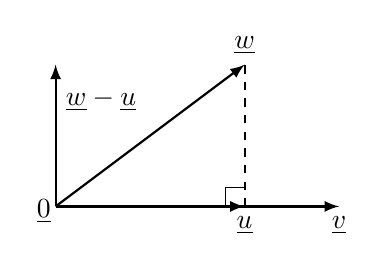
\begin{tikzpicture}[scale=0.6]
  \coordinate (v1) at (0,0);
  \coordinate (v2) at (4,3);
  \coordinate (v3) at (6,0);
  \coordinate (v4) at (4,0);
  \coordinate (v5) at (0,3);
  \path[draw] (3.6,0) -- (3.6,0.4) -- (4,0.4);
  \node (v0) at (-0.25,-0.1) {$\vecnot{0}$};
  \draw[-latex,thick] (v1) -- node[at end,above] {$\vecnot{w}$} (v2);
  \draw[-latex,thick] (v1) -- node[at end,below] {$\vecnot{v}$} (v3);
  \draw[-latex,thick] (v1) -- node[at end, below] {$\vecnot{u}$} (v4);
  \draw[thick,dashed] (v4) --  (v2);
  \draw[-latex,thick] (v1) -- node[right,near end] {$\vecnot{w}-\vecnot{u}$} (v5);
\end{tikzpicture}
\end{tabular}
\end{definition}

\end{frame}

\begin{frame}{3.6.1: Projection Lemma}

\vspace{-2mm}

\begin{lemma}
Let $\vecnot{u}$ be the projection of $\vecnot{w}$ onto $\vecnot{v}$.
Then, $\langle \vecnot{w}-\vecnot{u} | \vecnot{u} \rangle = 0$ and \vspace{-2mm}
\[ \|\vecnot{w}-\vecnot{u}\|^2 =  \|\vecnot{w}\|^2 - \| \vecnot{u} \|^2 = \|\vecnot{w}\|^2 - \frac{|\langle \vecnot{w} | \vecnot{v} \rangle|^2}{\|\vecnot{v}\|^2}. \]
\end{lemma}

\vspace{-1mm}

\begin{proof}<2->
First, we observe that \vspace{-3mm}
\[ \langle \vecnot{w} - \vecnot{u} | \vecnot{v} \rangle = \langle \vecnot{w} | \vecnot{v} \rangle - \langle \vecnot{u} | \vecnot{v} \rangle = \langle \vecnot{w} | \vecnot{v} \rangle - \frac{\left\langle \vecnot{w} | \vecnot{v} \right\rangle}{\|\vecnot{v}\|^2} \langle \vecnot{v} | \vecnot{v} \rangle = 0. \vspace{-1.5mm} \]
Since $\vecnot{u} = s \vecnot{v}$ for some scalar $s$, it follows that $\langle \vecnot{w}-\vecnot{u} | \vecnot{u} \rangle =  0$.
Using $\langle \vecnot{w}-\vecnot{u} | \vecnot{u} \rangle = 0$, we can write \vspace{-2mm}
\begin{align*}
\|\vecnot{w}\|^2 &= \|(\vecnot{w}-\vecnot{u})+\vecnot{u}\|^2
= \langle (\vecnot{w}-\vecnot{u})+\vecnot{u}|(\vecnot{w}-\vecnot{u})+\vecnot{u}\rangle \\
&= \|\vecnot{w}-\vecnot{u}\|^2 + 2 \Real \langle \vecnot{w}-\vecnot{u} | \vecnot{u} \rangle + \|\vecnot{u}\|^2
= \|\vecnot{w}-\vecnot{u}\|^2 + \|\vecnot{u}\|^2. \vspace{-1mm}
\end{align*}
The proof is completed by noting that $\|\vecnot{u}\|^2 = |\langle \vecnot{w} | \vecnot{v} \rangle|^2 / \|\vecnot{v}\|^2$.
\end{proof}

\end{frame}

\begin{frame}{3.6.1: Properties of the Induced Norm}

\begin{theorem}
If $V$ is an inner-product space over $F$ and $\| \vecnot{v} \| \triangleq \sqrt{\left\langle \vecnot{v} | \vecnot{v} \right\rangle}$, then for any $\vecnot{v}, \vecnot{w} \in V$ and any $s\in F$, it follows that
\begin{enumerate}
\item $\left\| s \vecnot{v} \right\| = |s| \left\| \vecnot{v} \right\|$
\item $\left\| \vecnot{v} \right\| > 0$ for $\vecnot{v} \neq \vecnot{0}$
\item $\left| \left\langle \vecnot{v} | \vecnot{w} \right\rangle \right| \leq \left\| \vecnot{v} \right\| \left\| \vecnot{w} \right\|$ with equality iff $\vecnot{v} = \vecnot{0}$, $\vecnot{w}=\vecnot{0}$, or $\vecnot{v} = s \vecnot{w}$
\item $\left\| \vecnot{v} + \vecnot{w} \right\| \leq \left\| \vecnot{v} \right\| + \left\| \vecnot{w} \right\|$ with equality iff $\vecnot{v} = \vecnot{0}$, $\vecnot{w}=\vecnot{0}$, or $\vecnot{v} = s \vecnot{w}$.
\end{enumerate}
\end{theorem}

\begin{proof}[Sketch of Proof]<2->
The first two follow immediately from definitions.
The third inequality, $\left| \left\langle \vecnot{v} | \vecnot{w} \right\rangle \right| \leq \left\| \vecnot{v} \right\| \left\| \vecnot{w} \right\|$, is called the \textcolor{blue}{Cauchy-Schwarz inequality}.
The fourth inequality is the triangle inequality for the induced norm and can be shown using the Cauchy-Schwarz inequality.
\end{proof}

\visible<2->{Proof of Cauchy-Schwarz in live session.}

\end{frame}

\begin{frame}{3.7: Sets of Orthogonal Vectors}

\vspace{-1mm}

\begin{definition}<1->
Let $V$ be an inner-product space and $U,W$ be subspaces.
Then, the subspace $U$ is an \textcolor{blue}{orthogonal} to the subspace $W$ (denoted $U \bot W$) if: \vspace{-2mm}
$$ \vecnot{u} \ \bot \, \vecnot{w} \text{  for all } \vecnot{u}\in U \text{ and } \vecnot{w}\in W. $$
\end{definition}

\vspace{-1mm}

\begin{definition}<2->
A subset $W\subset V$ of vectors is an \textcolor{blue}{orthogonal set} if all distinct pairs in $W$ are orthogonal.
A orthogonal set is \textcolor{blue}{orthonormal} if all vectors normalized.
\end{definition}

\vspace{-1mm}

\begin{example}<3->
For $\RealNumbers^n$ with standard inner product, the standard basis is an orthonormal.
\end{example}

\vspace{-1mm}

\begin{example}<4->
Let $V$ be the vector space (over $\ComplexNumbers$) of continuous functions $f\colon [0,1]\to\mathbb{C}$ with the standard inner product.
Let $f_n(x) = \sqrt{2} \cos 2 \pi n x$ and $g_n (x) = \sqrt{2} \sin 2 \pi n x$.
Then, $\{ 1, f_1, g_1, f_2, g_2, \ldots \}$ is a countably infinite orthonormal set and a Schauder basis for the closure of $V$.
\end{example}

\end{frame}

\begin{frame}{3.7: Properties of Orthogonal Sets}

\vspace{-1mm}

\begin{lemma}<1->
Let $V$ be an inner-product space and $W\subset V$ be an orthogonal set of non-zero vectors.
Let $\vecnot{v} = s_1 \vecnot{w}_1 + \cdots + s_n \vecnot{w}_n$ be a linear combination of distinct vectors in $W$.
Then, \vspace{-4mm}
\[ s_i = \frac{ \left\langle \vecnot{v} | \vecnot{w}_i \right\rangle }
{ \left\| \vecnot{w}_i \right\|^2 }\]
\end{lemma}

\vspace{-1mm}

\begin{proof}<2->
The inner product $\left\langle \vecnot{v} | \vecnot{w}_i \right\rangle$ is given by \vspace{-1.5mm}
\begin{equation*}
\begin{split}
\left\langle \vecnot{v} | \vecnot{w}_i \right\rangle
&= \left\langle \textstyle\sum_j s_j \vecnot{w}_j | \vecnot{w}_i \right\rangle
= \textstyle\sum_j s_j \left\langle \vecnot{w}_j | \vecnot{w}_i \right\rangle
= s_i \left\langle \vecnot{w}_i | \vecnot{w}_i \right\rangle .
\end{split} \vspace{-2.5mm}
\end{equation*}
Dividing both sides by $\| \vecnot{w}_i \|^2 = \left\langle \vecnot{w}_i | \vecnot{w}_i \right\rangle > 0$, gives the stated result.
\end{proof}

\begin{theorem}<3->
An orthogonal set of non-zero vectors is linearly independent.
\end{theorem}

\visible<3->{Proof by contradiction in live session.}

\end{frame}



\begin{frame}{3.7: Gram-Schmidt Orthogonalization (1)}

\vspace{-2mm}

\begin{block}{Gram-Schmidt Process}
Let $V$ be an inner-product space and assume $\vecnot{v}_1, \ldots, \vecnot{v}_n$ are linearly independent vectors in $V$.
Then, an orthogonal set of vectors $\vecnot{w}_1, \ldots, \vecnot{w}_n$ with the same span is produced by \textcolor{blue}{Gram-Schmidt process}:
\begin{enumerate}
\item Let $\vecnot{w}_1 = \vecnot{v}_1$

\item For $m=1,\ldots,n-1$, define \vspace{-4.5mm}
\begin{equation*}
\vecnot{w}_{m+1} = \vecnot{v}_{m+1} - \sum_{i=1}^m \frac{ \left\langle \vecnot{v}_{m+1} | \vecnot{w}_i \right\rangle } { \left\| \vecnot{w}_i \right\|^2 } \vecnot{w}_i.
\end{equation*}
\end{enumerate}
\end{block}

\vspace{-0,5mm}
\begin{itemize}
\setlength\itemsep{1.5mm}
\item<2-> Vector $\vecnot{w}_{m+1} \neq 0$. Otherwise, $\vecnot{v}_{m+1}$ is a linear combination of $\vecnot{w}_1, \ldots, \vecnot{w}_m$ and hence a linear combination of $\vecnot{v}_1, \ldots, \vecnot{v}_m$

\item<3-> Vectors $\vecnot{w}_{m+1}$ and $\vecnot{w}_j$ are orthogonal for $j=1,\ldots,m$: \vspace{-1.5mm}
\begin{equation*}
\begin{split}
\left\langle \vecnot{w}_{m+1} | \vecnot{w}_j \right\rangle
&= \left\langle \vecnot{v}_{m+1} | \vecnot{w}_j \right\rangle
- \sum_{i=1}^m \frac{ \left\langle \vecnot{v}_{m+1} | \vecnot{w}_i \right\rangle } { \left\| \vecnot{w}_i \right\|^2 }
\left\langle \vecnot{w}_i | \vecnot{w}_j \right\rangle \\
&= \left\langle \vecnot{v}_{m+1} | \vecnot{w}_j \right\rangle
- \frac{ \left\langle \vecnot{v}_{m+1} | \vecnot{w}_j \right\rangle } { \left\| \vecnot{w}_j \right\|^2 }
\left\langle \vecnot{w}_j | \vecnot{w}_j \right\rangle = 0
\end{split}
\end{equation*}

\end{itemize}

\end{frame}

\begin{frame}<1-3> \frametitle{3.7: Gram-Schmidt Orthogonalization (2)}

\vspace{-1.5mm}

\begin{example}
Let $V = \RealNumbers^3$ be the standard vector space equipped with the standard inner product and define \vspace{-4mm}
\begin{align*}
\vecnot{v}_1 &= (2,2,1) \\
\vecnot{v}_2 &= (3,6,0) \\
\vecnot{v}_3 &= (6,3,9)
\end{align*}
\vspace{-5mm}

Applying the Gram-Schmidt process to $\vecnot{v}_1, \vecnot{v}_2, \vecnot{v}_3$ results in: \vspace{-2mm}
\begin{align*}
\uncover<1->{\vecnot{w}_1 &= \textcolor{blue}{(2,2,1)} \\}
\uncover<2->{\vecnot{w}_2 &= (3,6,0)
- \frac{ \left\langle (3,6,0) | (2,2,1) \right\rangle }{ 9 } (2,2,1) \\}
\uncover<3->{&= (3,6,0) - 2 (2,2,1) = \textcolor{blue}{(-1,2,-2)} \\}
\uncover<4->{\vecnot{w}_3 &= \vecnot{v}_3
- \frac{ \left\langle (6,3,9) | (2,2,1) \right\rangle }{ 9 } (2,2,1)
- \frac{ \left\langle (6,3,9) | (-1,2,-2) \right\rangle }{ 9 } (-1,2,-2) \\}
\uncover<5->{&= (6,3,9) - 3 (2,2,1) + 2 (-1,2,-2) = \textcolor{blue}{(-2,1,2)}}
\end{align*}

\vspace*{-2mm}

\uncover<6->{It is easily verified that $\{ \vecnot{w}_1, \vecnot{w}_2, \vecnot{w}_3\}$ is an orthogonal set of vectors.}
\end{example}

\end{frame}


\begin{frame}{3.7: Orthogonal Complement}

\begin{definition}<1->
Let $V$ be an inner-product space and $W$ be any set of vectors in $V$.
The \textcolor{blue}{orthogonal complement} of $W$ denoted by $W^{\bot}$ is the set of all vectors in $V$ that are orthogonal to every vector in $W$ or \vspace{-2mm}
\begin{equation*}
W^{\bot} = \left\{ \vecnot{v} \in V \big| \langle \vecnot{v} | \vecnot{w} \rangle = 0 \; \forall \; \vecnot{w}\in W \right\}. 
\end{equation*}
\end{definition}

\begin{example}<2->
For the standard inner product space $V = \RealNumbers^3$, let subspace $U$ be spanned by \vspace{-2mm}
\begin{align*}
\vecnot{u}_1 &= (2,2,1) \\
\vecnot{u}_2 &= (3,6,0).
\end{align*}
\vspace*{-5.5mm}

Find the orthogonal complement $U^\perp$ of $U$.
\end{example}

\uncover<2->{Discussion in live session.}

\end{frame}


\begin{frame}{3.7.1: Hilbert Spaces}

\begin{definition}<1->
A complete inner-product space is called a \textcolor{blue}{Hilbert space}.
\end{definition}

\begin{example}<2->
Consider the Banach space $\ell^2$ of infinite real/complex sequences with Euclidean norm $\|\vecnot{v}\| = \left( \sum_{i=1}^\infty |v_i|^2 \right)^{1/2} < \infty$.
The set $\ell^2$ is a Hilbert space under the standard inner product because it induces the Euclidean norm.
\end{example}

\begin{theorem}<3->
If Hilbert space $V$ has a countable dense subset, then there is a linear transform $T:V\to \ell^2$ such that $\left\langle \vecnot{u} | \vecnot{v} \right\rangle_V = \left\langle T\vecnot{u} | T\vecnot{v} \right\rangle_{\ell^2}$ for all $\vecnot{u},\vecnot{v} \in V$.
\end{theorem}

\uncover<3->{Thus, any separable Hilbert space is equivalent to the Hilbert space $\ell^2$.}

%\begin{example}[Quantum Mechanics]
%Quantum mechanics is derived in the Hilbert space $\ell^2$ because:
%\begin{itemize}
%\item the state of a closed $n$-dimensional quantum systems is modeled by a unit vector in the standard inner product space for $\mathbb{C}^n$
%\item all allowable operations on the system result either in unitary evolution or a known projection of that vector
%\item sequentially joining the states of all quantum systems in the universe gives a sequence of state vectors of dimension tending to infinity
%\end{itemize}
%\end{example}

\end{frame}


\begin{frame}{3.7: Unitary Matrices}

\vspace{-1.5mm}

\begin{definition}<1->
A complex matrix $U\in \ComplexNumbers^{n\times n}$ is called \textcolor{blue}{unitary} if $U^H U = I$.
Similarly, a real matrix $Q\in \RealNumbers^{n\times n}$ is called \textcolor{blue}{orthogonal} if $Q^T Q = I$.
\end{definition}

\vspace{-1.5mm}

\begin{theorem}<2->
Let $V = \ComplexNumbers^n$ be the standard inner product space and let  $U\in \ComplexNumbers^{n\times n}$ define a linear operator on $V$.
Then, the following conditions are equivalent:
\begin{enumerate}
\setlength\itemsep{0.5mm}
\item[(i)] The columns of $U$ form an orthonormal basis (i.e.,  $U^H U = I$),
\item[(ii)] the rows of $U$ form an orthonormal basis (i.e.,  $U U^H = I$),
\item[(iii)] $U$ preserves inner products (i.e., $\langle U \vecnot{v} | U \vecnot{w} \rangle = \langle \vecnot{v} | \vecnot{w} \rangle$ for all $\vecnot{u},\vecnot{v}\in V$),
\item[(iv)] $U$ is an isometry (i.e., $\| U \vecnot{v} \| = \| \vecnot{v}\|$ for all $\vecnot{v} \in V$).
\end{enumerate}
\end{theorem}

\vspace{-1.5mm}

\begin{proof}<3->
{\it(i)}$\Rightarrow${\it(ii)}: Orthogonal columns implies $U$ invertible and $U^H U = I$ implies $U^H = U^{-1}$.
{\it(i)}$\Rightarrow${\it(iii)}: $\langle U \vecnot{v} | U \vecnot{w} \rangle = \vecnot{w}^H U^H U \vecnot{v} = \vecnot{w}^H \vecnot{v} = \langle \vecnot{v} | \vecnot{w} \rangle$ and $\vecnot{w}=\vecnot{v}$ gives {\it(iv)}.
{\it(iv)}$\Rightarrow${\it(i)}:
$\vecnot{v}^H (U^H U \!-\! I) \vecnot{v} \!=\! \| U \vecnot{v} \|^2 \!-\! \| \vecnot{v} \|^2 \!=\! 0$
%because $\| U \vecnot{v} \| \!=\! \| \vecnot{v}\|$
and, as $U^H U \!-\! I$ is Hermitian, all eigenvalues are 0 and $U^H U - I = 0$.
\end{proof}

\end{frame}


\begin{frame}{3.8: Linear Functionals and the Riesz Theorem}

\begin{definition}
Let $V$ be a vector space over a field $F$.
A linear transformation $f$ from $V$ into the scalar field $F$ is called a \textcolor{blue}{linear functional} on $V$.
\end{definition}

\begin{example}
Thus, $f\colon V \to F$ is a function on $V$ such that
\begin{equation*}
f \left( s \vecnot{v}_1 + \vecnot{v}_2 \right)
= s f \left( \vecnot{v}_1 \right) + f \left( \vecnot{v}_2 \right)
\end{equation*}
for all $\vecnot{v}_1, \vecnot{v}_2 \in V$ and $s \in F$.
\end{example}

\begin{theorem}[Riesz]
Let $V$ be a Hilbert space and $f$ be a continuous linear functional on $V$.
Then, there exists a unique vector $\vecnot{v} \in V$ such that $f \left( \vecnot{w} \right) = \left\langle \vecnot{w} | \vecnot{v} \right\rangle$ for all $\vecnot{w} \in V$.
\end{theorem}

\end{frame}



\begin{frame} \frametitle{Next Steps}

\begin{itemize}
\setlength\itemsep{5mm}
\item To continue studying after this video -- \vspace{2mm}

\begin{itemize}
 \setlength\itemsep{3mm}
 \item Try the required reading: Course Notes EF 3.6 - 3.8
 \item Or the recommended reading: LADR 6AB
 \item Also, look at the problems in Assignment 6
\end{itemize}
\end{itemize}

\note{
	\vspace{8mm}
	\begin{enumerate}
		\setlength\itemsep{3mm}
		\color{red}
		\item Here are some options to continue learning this material. (read) \\ [2mm]  That's it for today.  So, I'll see you next time.
	\end{enumerate}
}

\end{frame}


\end{document}


\begin{frame}{Derivatives in Banach Spaces}

The foundation of engineering is the ability to use math and physics to design and optimize complex systems.

\vspace{3mm}

Computers have now made this possible on an unprecedented scale.

\vspace{3mm}

In vector analysis, derivatives are usually introduced using Banach spaces: \vspace{-2mm}
\begin{itemize}
\item<1-> For a function $f \colon X \rightarrow Y$, the definition of the derivative requires a linear structure (to define differences) and a topology (to define convergence) on both $X$ and $Y$ \vspace{1mm}

\item<2-> If $X=\RealNumbers^n$ and $Y=\RealNumbers^m$, then the derivative is a linear transform from $X$ to $Y$ represented by the Jacobian matrix $f'(\vecnot{x}) \in \RealNumbers^{m\times n}$ \vspace{1mm}

\item<3-> Thus, we generally assume $f \colon X \rightarrow Y$ be a mapping from the Banach space $(X,\|\cdot\|_X)$ to the Banach space $(Y,\|\cdot\|_Y)$ \vspace{1mm}

\item<4-> For directional derivatives, one only needs the linear structure on $X$
\end{itemize}
\end{frame}

\begin{frame}{Directional Derivatives}

\begin{definition}[Directional Derivative]<1->
Let $f \colon X \rightarrow Y$ map vector space $X$ to a Banach space $(Y,\|\cdot\|)$.
Then, if it exists, the \textcolor{blue}{G\^{a}teaux differential} of $f$ at  $\vecnot{x}$ in direction $\vecnot{h}$ is given by \vspace{-1.5mm}
\[ \delta f (\vecnot{x};\vecnot{h}) \triangleq \lim_{t \to 0} \frac{f(\vecnot{x}+t \vecnot{h}) - f(\vecnot{x})}{t}. \]
%where the limit is with respect to the implied mapping from $\RealNumbers$ to $Y$.
\end{definition}

\begin{example}<2->
Consider $X\!=\!Y\!=\!\mathbb{R}^2$ and $f(\vecnot{x})\! =\! (x_1 x_2,x_1+x_2^2)$.
For $\vecnot{x}\!=\!(1,1)$, $\vecnot{h}\!=\!(1,2)$: \vspace{-2.5mm}
\[ \delta f ( \vecnot{x},\vecnot{h} ) = \frac{d}{dt} ((1+t)(1+2t),(1+t)+(1+2t)^2) \Big|_{t=0} = (3,5). \]
\end{example}

\begin{lemma}<3->
Let $Y=\RealNumbers$ and suppose that $\delta f (\vecnot{x};\vecnot{h})$ exists and is negative for some $f$, $\vecnot{x}$, and $\vecnot{h}$.  Then, there exists $t_0 > 0$ such that, for all $t\in(0,t_0)$, one has \vspace{-2mm}
\[ f(\vecnot{x}+t \vecnot{h}) < f (\vecnot{x}). \]
\end{lemma}

\visible<3->{Proof on whiteboard.}

\end{frame}

\begin{frame}{What is Meant by Differentiable?}

\begin{definition}
Let $f \colon X \rightarrow Y$ be a mapping from a vector space $X$ to a Banach space $(Y,\|\cdot\|)$.
Then, $f$ is \textcolor{blue}{G\^{a}teaux differentiable} at $\vecnot{x}$ if the G\^{a}teaux differential $\delta f (\vecnot{x};\vecnot{h})$ exists for all $\vecnot{h} \in X$ and is a continuous linear function of $\vecnot{h}$.
\end{definition}

\begin{definition}[Differentiable]
Let $f \colon X \rightarrow Y$ be a mapping from a Banach space $(X,\|\cdot\|_X)$ to a Banach space $(Y,\|\cdot\|_Y)$.
Then, $f$ is \textcolor{blue}{Fr\'{e}chet differentiable} at $\vecnot{x}$ if there is a continuous linear transformation $T\colon X \to Y$ satisfying
\begin{equation*} \lim_{\vecnot{h} \to \vecnot{0}} \frac{\left\|f(\vecnot{x}+ \vecnot{h}) - f(\vecnot{x}) - T(\vecnot{h}) \right\|_Y}{\| \vecnot{h} \|_X} = 0,
\end{equation*}
where the limit is with respect to the implied Banach space mapping $X\to \RealNumbers$.
In this case, the \textcolor{blue}{Fr\'{e}chet derivative} $f'(\vecnot{x})$ equals $T$.
\end{definition}
\end{frame}

\begin{frame}{Gradient Descent}

\begin{itemize}
\item<1-> Gradient descent subtracts the gradient $\nabla f(\vecnot{x})$ from an element of $X\!\!\!$ \vspace{1mm}

\item<2-> But, for a Banach space, the derivative is a linear functional mapping $X$ to $\RealNumbers$!

\item<3-> How can one add a linear mapping to $X$?

\item<4-> In Hilbert space, the Riesz representation theorem states every linear functional is represented by the inner product with a fixed vector

\item<5-> Thus, the gradient $\nabla f (\vecnot{x}) \in X$ is defined as the representative vector
\end{itemize}

\begin{definition}[Gradient Descent]<6->
Let $f \colon X \rightarrow \RealNumbers$ be a mapping from a Hilbert space $X$ to the standard Banach space of real numbers.
Starting from $\vecnot{x}_1 \in X$, \textcolor{blue}{gradient descent} defines the sequence \vspace{-4mm}
\[ \vecnot{x}_{n+1} = \vecnot{x}_n - \delta_n \nabla f(\vecnot{x}_n), \]
where $\delta_n$ is the step size and the gradient $\nabla f (\vecnot{x})$ is uniquely defined by \vspace{-1.5mm}
\[\langle \vecnot{h} | \nabla f(\vecnot{x}) \rangle = f'(\vecnot{x})(\vecnot{h}) \text{ for all } \vecnot{h} \in X. \]
\end{definition}


\end{frame}


\backupbegin

%\begin{frame}
%\frametitle{Backup Slides}
%\begin{itemize}
%\item Slide numbers not included in denominator!
%\end{itemize}
%\end{frame}

%\begin{frame}[allowframebreaks]
%\frametitle{References}
%\bibliographystyle{alpha}
%\footnotesize
%\bibliography{IEEEabrv,WCLabrv,WCLbib,WCLnewbib}
%\end{frame}

\backupend

\end{document}
